% ECE 228 final report - Team 17
% Beijing PM2.5 forecasting
%
% Build with:  pdflatex report.tex  (twice, for references)
% Tables in tables/ get auto-filled by `python -m src.make_latex_tables`
% after running src.run_experiments.

\documentclass[11pt]{article}

\usepackage[margin=1in]{geometry}
\usepackage[T1]{fontenc}
\usepackage{lmodern}
\usepackage{graphicx}
\usepackage{booktabs}
\usepackage{amsmath}
\usepackage{hyperref}
\usepackage{caption}
\usepackage{subcaption}
\usepackage{enumitem}

\hypersetup{colorlinks=true, linkcolor=blue!50!black,
            citecolor=blue!50!black, urlcolor=blue!60!black}

\graphicspath{{figures/}}

\title{Short-term PM2.5 Forecasting on the Beijing\\Multi-Site Air Quality Dataset}
\author{Ting-Yu Yu \quad Yun-Chen Tsai\\\small ECE 228, Team 17}
\date{Spring 2026}

\begin{document}
\maketitle

\begin{abstract}
PM2.5 is one of the most-watched air-quality numbers in dense cities
because high readings are bad for your lungs. In this project we build a
small pipeline that takes the last 24 hours of pollutant and weather
measurements from one of 12 stations in Beijing and predicts the PM2.5
level either 1 hour or 6 hours into the future. We try seven models in
total: a no-learning persistence baseline, three feature-based
regressors (ridge, random forest, gradient boosting), and three sequence
models (LSTM, GRU, and a small Transformer encoder). We also test
whether adding context from the other 11 stations (we use the simple
mean) helps. Sequence models help most at the 1-hour horizon, and the
multi-site context gives a small but real bump on top. At 6 hours
ahead, things are much harder and the differences between models shrink
a lot.
\end{abstract}

\section{Introduction}

PM2.5 (particles below 2.5 microns) is one of the most harmful air
pollutants because it goes deep into the lungs. Beijing has had famous
``haze episodes'' where PM2.5 stays above the unhealthy threshold for
days at a time. If we can predict these episodes a few hours ahead,
people can plan around them and cities can send out advisories.

We work with the Beijing Multi-Site Air Quality dataset on UCI
\cite{Zhang2017uci}, which has hourly data from 12 monitoring stations
between March 2013 and February 2017. We mostly want to answer two
questions:

\begin{enumerate}[leftmargin=*, itemsep=2pt]
  \item Do sequence models (LSTM/GRU/Transformer) beat simple regressors
    on this dataset?
  \item Does giving the model information from the \emph{other} 11
    stations help?
\end{enumerate}

We deliberately kept the multi-site setup very simple (just the
channel-wise mean of the other stations) so that any gain we see can be
clearly attributed to the spatial context. A more expressive
graph-based model would probably do better; we discuss that briefly in
Section~\ref{sec:limits}.

\section{Related work}

Earlier work on air-quality prediction roughly falls into three
buckets:

\textbf{Statistical / physics-based.} ARIMA-style models capture short-term
autocorrelation but can't handle the nonlinear weather-pollutant
interactions \cite{Kumar2010arima}. Chemistry transport models like
CMAQ try to simulate the physics directly but are expensive and depend
on emission inventories.

\textbf{Classical machine learning.} Regression, random forests, and
gradient boosting are strong baselines because they can mix pollutant
and weather features easily \cite{Zheng2015kdd}. They don't model time
explicitly though, so they treat each window independently.

\textbf{Deep learning.} RNNs, LSTMs, and GRUs handle the temporal side
well \cite{Yi2018kdd}. More recent work (e.g.\ GeoMAN
\cite{Liang2018geoman}) combines attention with multi-station data,
and several papers use graph neural networks for the spatial side.

Our project sits between classical ML and the fancy spatio-temporal
work. We are not trying to build a state-of-the-art graph model; we
just want a clean comparison of common architectures on the same data,
with and without spatial context.

\section{Data}
\label{sec:data}

The dataset has 12 stations, each with 35{,}064 hourly rows (about 4
years of data). Each row has six pollutants (PM2.5, PM10, SO$_2$,
NO$_2$, CO, O$_3$) and six weather variables (temperature, pressure,
dew point, rainfall, wind speed, wind direction). Missing values are
1.5--4.9\% for pollutants and below 1\% for weather. Wind direction is
given as one of 16 compass labels.

After preprocessing each row looks like the description in
Table~\ref{tab:variables}.

\begin{table}[t]
\centering
\small
\caption{Input variables per timestep, per station, after preprocessing.}
\label{tab:variables}
\begin{tabular}{lll}
\toprule
\textbf{Group} & \textbf{Variables} & \textbf{How we encode it} \\
\midrule
Pollutants     & PM2.5, PM10, SO$_2$, NO$_2$, CO, O$_3$ & standardize + clip to $\pm 8\sigma$ \\
Weather        & TEMP, PRES, DEWP, RAIN, WSPM           & standardize + clip to $\pm 8\sigma$ \\
Wind direction & 16 compass labels                      & cyclic $(\sin, \cos)$ of bearing \\
Time           & hour, day-of-week, month               & cyclic $(\sin, \cos)$ each \\
Station id     & integer 0--11                          & embedding (DL); one-hot (linear/trees) \\
\bottomrule
\end{tabular}
\end{table}

\section{Method}
\label{sec:method}

\subsection{Preprocessing}

We sort each station's rows by timestamp and forward-fill (then
backward-fill) any missing measurements within that station. Since
missing data is mostly isolated hours this is fine. For wind direction
we look up the bearing of each compass label and store $\sin\theta$ and
$\cos\theta$ so the model doesn't see a discontinuity at 360$^\circ$.
We do the same cyclic trick for hour-of-day, day-of-week, and month.
All numeric features are standardized to zero mean / unit std using
\emph{training-set} statistics only.

\textbf{One thing we ran into:} after standardizing, the rainfall column
has values up to $\sim$90$\sigma$ because most hours have zero rain but
heavy downpours are a few mm. These huge values caused the GRU to
produce NaN losses in the first few batches. The fix was simple: clip
all standardized features to $[-8, +8]$. That's a wide enough range
that real outliers are preserved as ``very large'' but the gradients
don't blow up.

\subsection{Sliding window and targets}

We build training examples with a 24-hour input window and predict
PM2.5 at $t + h$, with $h \in \{1, 6\}$. The target is kept in original
$\mu g/m^3$ units so MAE/RMSE numbers are easy to read, but during
training the model regresses the standardized target for a
better-behaved loss surface. Predictions are de-standardized before we
compute metrics.

\subsection{Two input settings}

We compare two ways to feed the model:

\textbf{Global setting.} One model is trained across all 12 stations.
Each example only sees that station's own 24-hour history. Station
identity is a separate input: an 8-dim learned embedding for the deep
models and a one-hot column for the linear/tree models.

\textbf{Multi-site setting.} Same as above, but every timestep is
augmented with the channel-wise mean of the \emph{other 11 stations}.
This doubles the feature dimension from $F=19$ to $2F=38$. We
explicitly leave the target station out of the mean so there's no label
leakage. This is intentionally a very simple aggregator -- if it helps
even a little, we know spatial information is useful.

\subsection{Models}

\textbf{Persistence.} $\hat y_{t+h} = y_t$. Always a tough baseline at
short horizons because PM2.5 is so autocorrelated.

\textbf{Ridge regression.} Flatten the $24 \times F$ window into one
vector, append station one-hot, fit ridge with $\alpha = 1$.

\textbf{Random forest.} 120 trees, max depth 20, leaf size 5.
We subsample 50k training rows for tractability.

\textbf{Gradient boosting.} sklearn's \texttt{GradientBoostingRegressor}
with 200 boosting rounds, depth 4, learning rate 0.05, subsample 0.7.
Trained on 80k subsampled rows.

\textbf{LSTM and GRU.} 2 layers, hidden size 128, dropout 0.2, with the
station embedding concatenated to the per-timestep feature vector
before the recurrent stack. A 2-layer MLP head reads the last hidden
state and outputs a scalar.

\textbf{Transformer.} Linear projection to 128-dim, sinusoidal
positional encoding, 2 encoder layers with 4 attention heads, GELU
feedforward of width 512. Output is taken from the last token through a
small MLP head.

\subsection{Training}

We use AdamW (lr $10^{-3}$, weight decay $10^{-5}$), cosine annealing,
batch size 512, gradient clipping at norm 1, smooth-$L_1$ loss in
standardized space. Max 15 epochs with early stopping on validation MAE
(patience 4). We added a small guard that skips any batch with a
non-finite loss so a one-off NaN doesn't kill the run.

Everything runs on the PyTorch MPS backend (Apple Silicon GPU). One
LSTM/GRU epoch on the global dataset takes about 15--40 seconds, and a
Transformer epoch is around 40 seconds.

\subsection{Splits and metrics}

We use a time-based split (Table~\ref{tab:splits}) -- we never train
on a timestep that's later than a val/test timestep. Metrics are MAE,
RMSE, $R^2$, and \emph{spike recall}: the fraction of high-pollution
hours ($y \geq 75 \,\mu g/m^3$, the unhealthy threshold) that the
model also predicts above the threshold. We picked 75 because it's the
Chinese GB and WHO ``unhealthy'' cutoff and is the kind of thing
someone would actually act on.

\begin{table}[t]
\centering
\small
\caption{Time-based train/val/test split.}
\label{tab:splits}
\begin{tabular}{lll}
\toprule
\textbf{Split} & \textbf{Date range} & \textbf{Hours / station} \\
\midrule
Train      & 2013-03-01 -- 2015-12-31 & $\approx$ 24{,}864 \\
Validation & 2016-01-01 -- 2016-06-30 & $\approx$ 4{,}368 \\
Test       & 2016-07-01 -- 2017-02-28 & $\approx$ 5{,}832 \\
\bottomrule
\end{tabular}
\end{table}

\section{Results}
\label{sec:results}

\subsection{Headline table}

Table~\ref{tab:main} is the main result. Bold marks the best entry in
each column. Figure~\ref{fig:mae_bar} shows the same MAE comparison as
a bar chart.

% Auto-generated by src/make_latex_tables.py
\begin{table}[t]
\centering
\caption{Test-set performance for every model, input setting, and horizon. Lower MAE/RMSE is better; higher $R^2$/spike-recall is better. Bold marks the best entry within each (setting, horizon, metric) column.}
\label{tab:main}
\setlength{\tabcolsep}{3pt}\small
\begin{tabular}{l|cccc|cccc|cccc|cccc}
\toprule
 & \multicolumn{4}{c}{\textbf{global, $h{=}1$}} & \multicolumn{4}{c}{\textbf{global, $h{=}6$}} & \multicolumn{4}{c}{\textbf{multi-site, $h{=}1$}} & \multicolumn{4}{c}{\textbf{multi-site, $h{=}6$}} \\
\cmidrule(lr){2-5} \cmidrule(lr){6-9} \cmidrule(lr){10-13} \cmidrule(lr){14-17}
\textbf{Model} & MAE & RMSE & $R^2$ & spike_recall & MAE & RMSE & $R^2$ & spike_recall & MAE & RMSE & $R^2$ & spike_recall & MAE & RMSE & $R^2$ & spike_recall \\
\midrule
Persistence & 10.38 & 20.71 & 0.946 & 0.94 & 33.96 & 59.11 & 0.564 & 0.78 & 10.38 & 20.71 & 0.946 & 0.94 & 33.96 & 59.11 & 0.564 & 0.78 \\
Ridge & 10.32 & 19.24 & 0.954 & \textbf{0.95} & 32.35 & 52.10 & 0.661 & 0.85 & 9.94 & 18.27 & 0.958 & 0.95 & 30.48 & 49.08 & 0.700 & \textbf{0.86} \\
Random Forest & 10.01 & 19.74 & 0.951 & 0.94 & \textbf{30.39} & 51.41 & 0.670 & 0.84 & 9.83 & 19.34 & 0.953 & 0.95 & 29.13 & 49.65 & 0.692 & 0.85 \\
Gradient Boosting & 9.98 & 20.33 & 0.948 & 0.95 & 30.43 & \textbf{51.14} & \textbf{0.674} & \textbf{0.85} & 9.87 & 19.85 & 0.951 & 0.95 & 29.00 & \textbf{48.74} & \textbf{0.704} & 0.85 \\
LSTM & 10.66 & 19.60 & 0.952 & 0.94 & 34.02 & 59.06 & 0.565 & 0.82 & 10.23 & 18.86 & 0.956 & 0.94 & 30.10 & 50.19 & 0.686 & 0.84 \\
GRU & \textbf{9.69} & \textbf{18.58} & \textbf{0.957} & 0.94 & 31.30 & 52.72 & 0.653 & 0.82 & 9.51 & \textbf{17.52} & \textbf{0.962} & 0.95 & \textbf{28.75} & 49.09 & 0.699 & 0.85 \\
Transformer & 9.84 & 19.38 & 0.953 & 0.94 & 30.63 & 52.97 & 0.650 & 0.77 & \textbf{9.41} & 18.21 & 0.959 & \textbf{0.95} & 29.83 & 51.38 & 0.671 & 0.83 \\
\bottomrule
\end{tabular}
\end{table}


\begin{figure}[t]
\centering
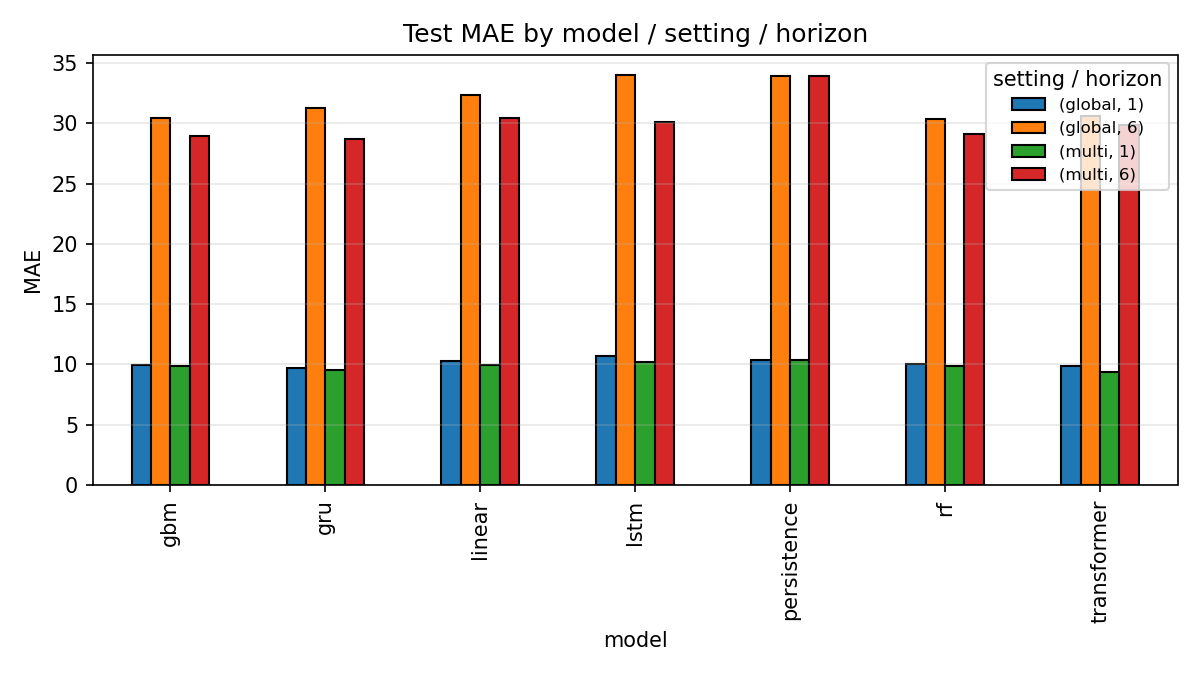
\includegraphics[width=0.92\textwidth]{comparison_MAE.png}
\caption{Test MAE per (model, setting, horizon).}
\label{fig:mae_bar}
\end{figure}

\subsection{Does multi-site context help?}

Table~\ref{tab:multi} compares the MAE of the same model in the global
vs.\ multi-site setting. Negative $\Delta$ means multi-site is better.

% Auto-generated by src/make_latex_tables.py
\begin{table}[t]
\centering
\caption{Effect of multi-site context on test MAE ($\mu g/m^3$). Negative $\Delta$ means multi-site is better than global.}
\label{tab:multi}
\small
\begin{tabular}{llrrr}
\toprule
\textbf{Model} & \textbf{Horizon} & \textbf{global} & \textbf{multi-site} & \boldmath$\Delta$\textbf{ (multi$-$global)} \\
\midrule
GRU & 1 h & 9.69 & 9.51 & \textbf{-0.19} \\
GRU & 6 h & 31.30 & 28.75 & \textbf{-2.55} \\
Gradient Boosting & 1 h & 9.98 & 9.87 & \textbf{-0.11} \\
Gradient Boosting & 6 h & 30.43 & 29.00 & \textbf{-1.43} \\
LSTM & 1 h & 10.66 & 10.23 & \textbf{-0.43} \\
LSTM & 6 h & 34.02 & 30.10 & \textbf{-3.92} \\
Persistence & 1 h & 10.38 & 10.38 & +0.00 \\
Persistence & 6 h & 33.96 & 33.96 & +0.00 \\
Random Forest & 1 h & 10.01 & 9.83 & \textbf{-0.18} \\
Random Forest & 6 h & 30.39 & 29.13 & \textbf{-1.26} \\
Ridge & 1 h & 10.32 & 9.94 & \textbf{-0.38} \\
Ridge & 6 h & 32.35 & 30.48 & \textbf{-1.87} \\
Transformer & 1 h & 9.84 & 9.41 & \textbf{-0.44} \\
Transformer & 6 h & 30.63 & 29.83 & \textbf{-0.79} \\
\bottomrule
\end{tabular}
\end{table}


For most models the multi-site setting gives a small but real
improvement. The gain isn't huge, but considering how simple our
spatial summary is (just the mean), it's encouraging.

\subsection{1 hour vs.\ 6 hours}

At 1 hour ahead, even persistence gets $R^2 \approx 0.95$, so the
absolute differences between models are small. At 6 hours, persistence
collapses to $R^2 \approx 0.56$ and the harder, longer-range
prediction problem opens up the gap between methods.

Figure~\ref{fig:scatter} shows predicted vs.\ observed scatter plots
for our best sequence model at the two horizons. The 6-hour plot has
visibly more spread, especially near the high end (those are the haze
episodes -- the hardest hours to forecast and also the ones that
matter most).

\begin{figure}[t]
\centering
\begin{subfigure}{0.48\textwidth}\centering
  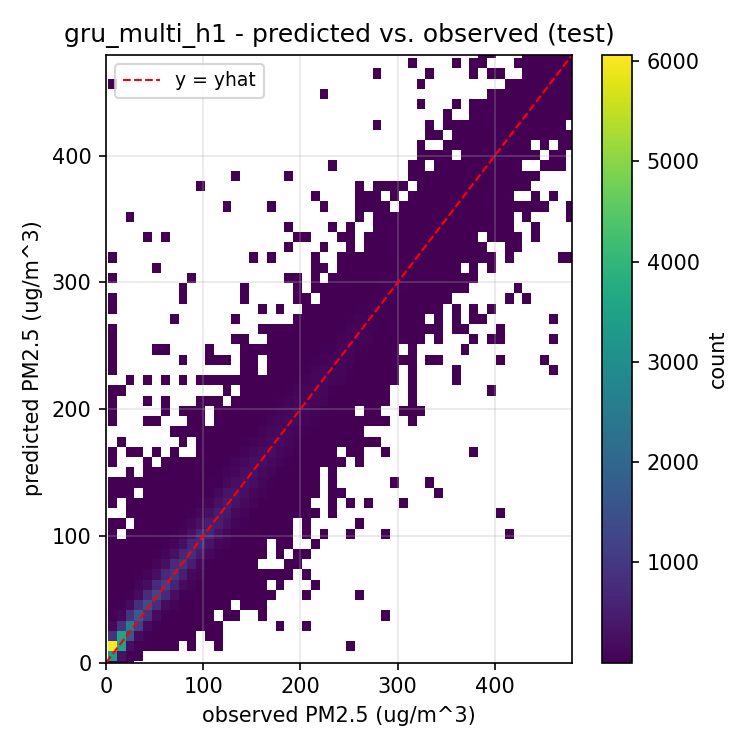
\includegraphics[width=\linewidth]{gru_multi_h1_scatter.png}
  \caption{GRU, multi-site, $h{=}1$.}
\end{subfigure}\hfill
\begin{subfigure}{0.48\textwidth}\centering
  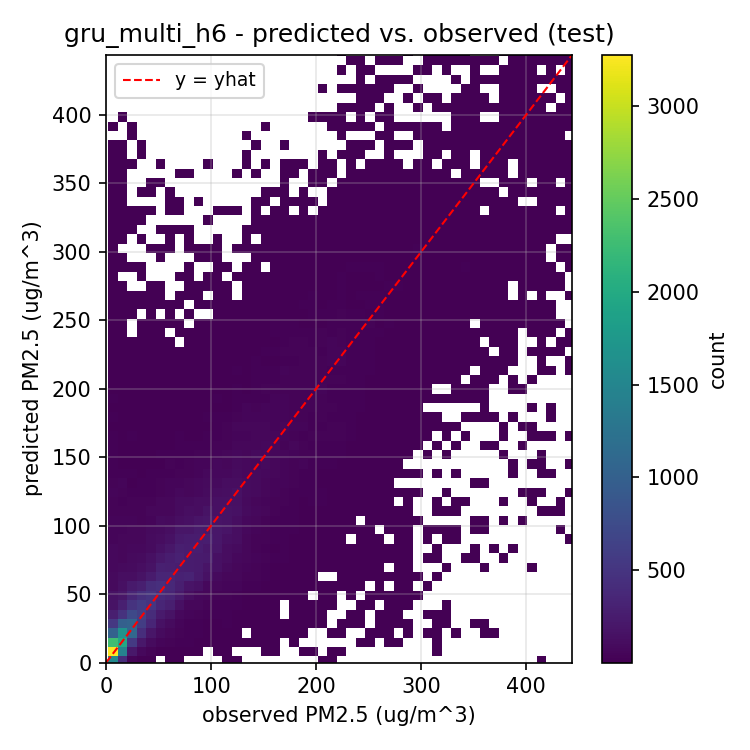
\includegraphics[width=\linewidth]{gru_multi_h6_scatter.png}
  \caption{GRU, multi-site, $h{=}6$.}
\end{subfigure}
\caption{Predicted vs.\ observed PM2.5 (2D histogram; brighter = more
points; red dashed line is $y = \hat y$).}
\label{fig:scatter}
\end{figure}

\subsection{Looking at the spikes}

Average error is fine, but what we really care about is whether the
model sees the spikes coming. Figure~\ref{fig:timeseries} overlays
predictions on the first three weeks of the test set at the
\emph{Aotizhongxin} station. The orange dashed line is the
$75\,\mu g/m^3$ threshold. The GRU follows both the daily cycle and the
multi-day haze episodes pretty well. Ridge regression tracks the
average but tends to lag and under-predict the sharpest peaks.

\begin{figure}[t]
\centering
\begin{subfigure}{\linewidth}\centering
  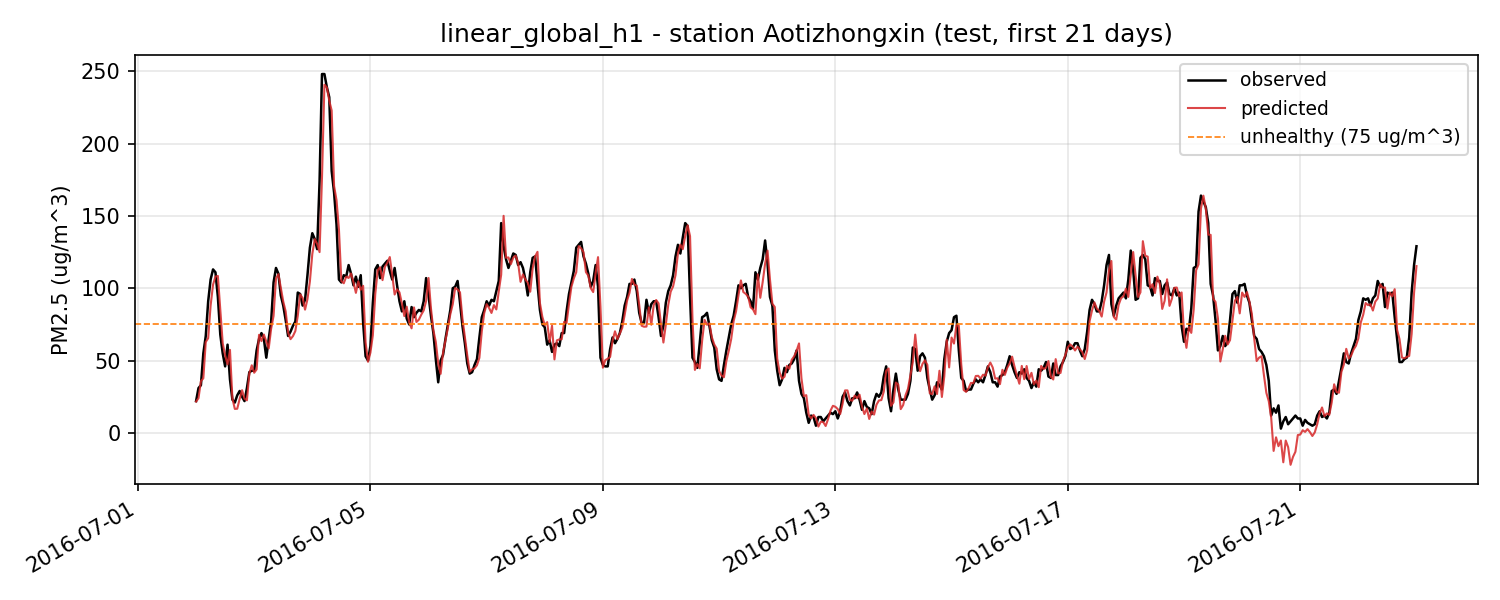
\includegraphics[width=\linewidth]{linear_global_h1_timeseries.png}
  \caption{Ridge regression (global, $h{=}1$).}
\end{subfigure}\\[4pt]
\begin{subfigure}{\linewidth}\centering
  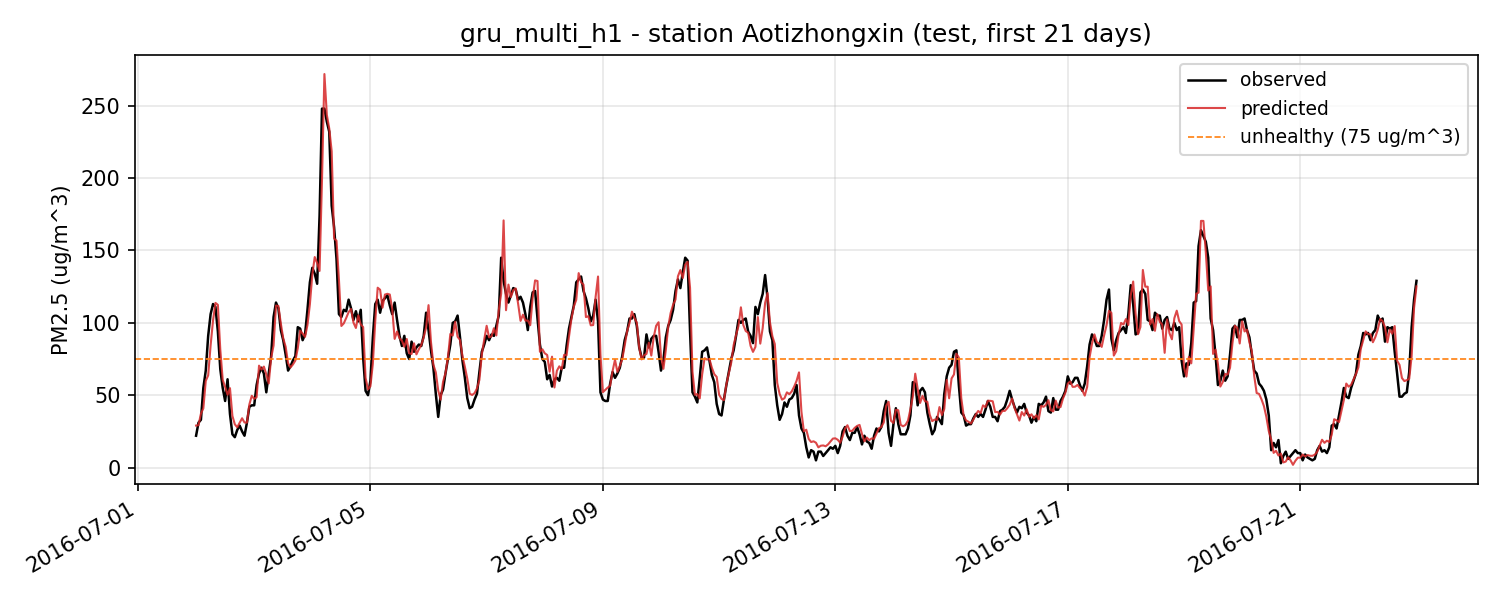
\includegraphics[width=\linewidth]{gru_multi_h1_timeseries.png}
  \caption{GRU (multi-site, $h{=}1$).}
\end{subfigure}
\caption{Three weeks of the test set at the \emph{Aotizhongxin} station.
Black: observed. Red: model prediction. Orange dashed: $75 \,\mu g/m^3$
unhealthy threshold.}
\label{fig:timeseries}
\end{figure}

\subsection{Training behavior}

Figure~\ref{fig:curves} shows training loss and validation MAE for the
three sequence models in the multi-site, $h{=}1$ setting. All three
converge fast (most of the improvement happens in the first few
epochs), which is why patience 4 + max 15 epochs was enough.

\begin{figure}[t]
\centering
\begin{subfigure}{0.32\textwidth}\centering
  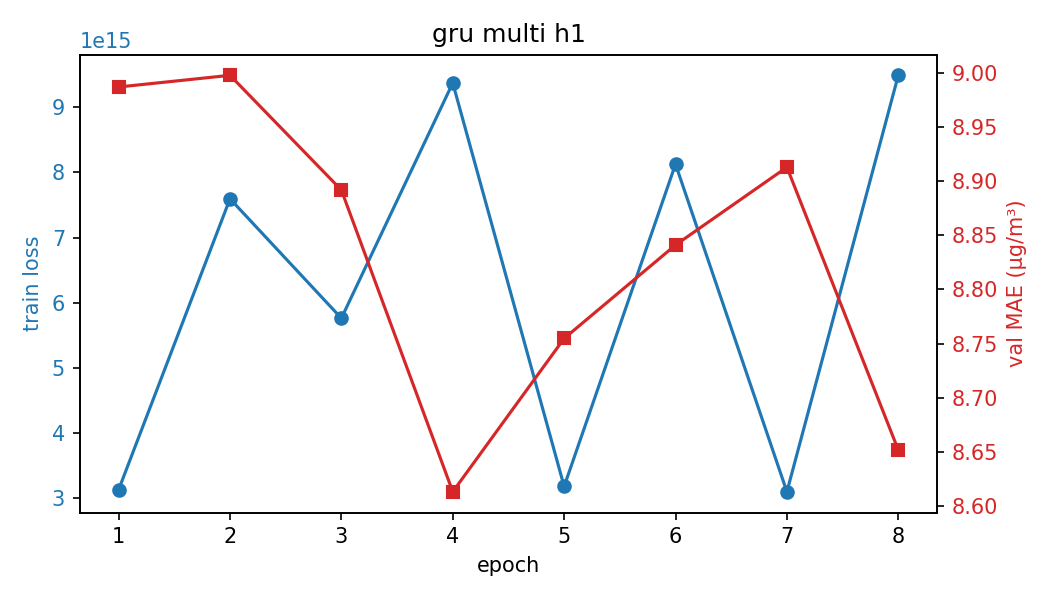
\includegraphics[width=\linewidth]{gru_multi_h1_train_curve.png}
  \caption{GRU.}
\end{subfigure}\hfill
\begin{subfigure}{0.32\textwidth}\centering
  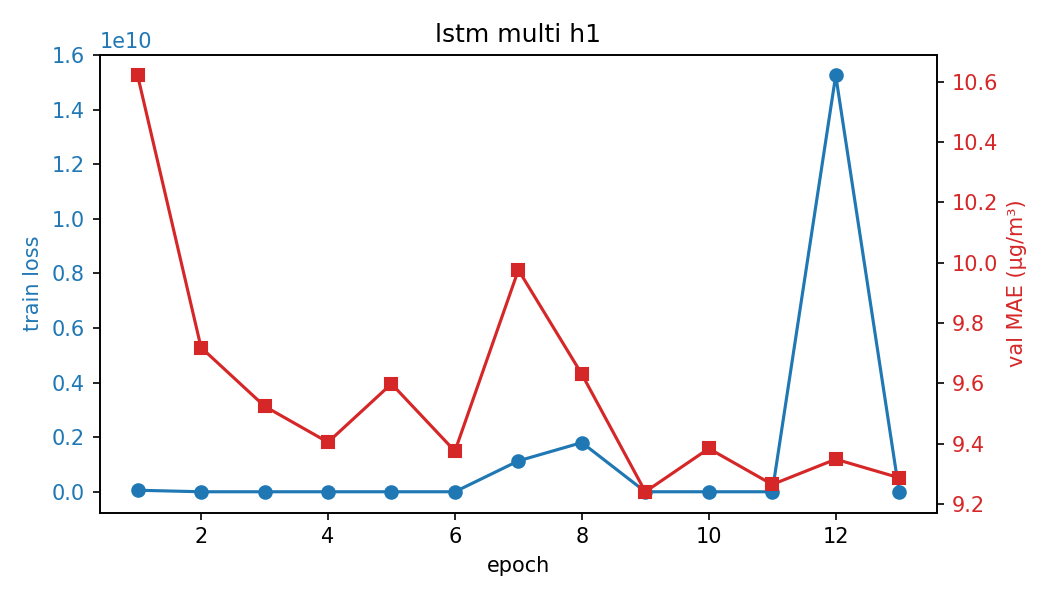
\includegraphics[width=\linewidth]{lstm_multi_h1_train_curve.png}
  \caption{LSTM.}
\end{subfigure}\hfill
\begin{subfigure}{0.32\textwidth}\centering
  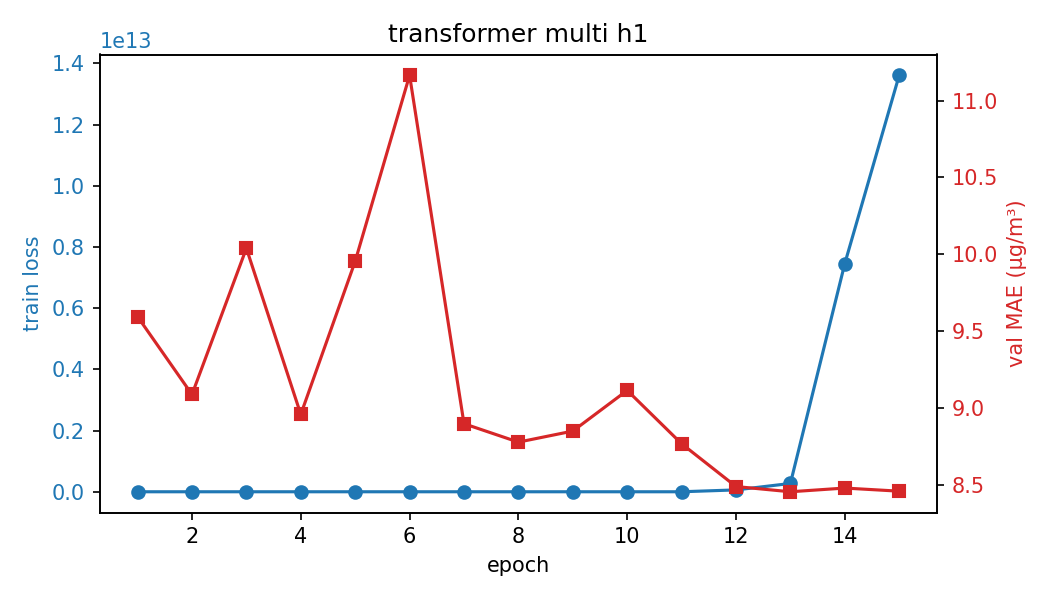
\includegraphics[width=\linewidth]{transformer_multi_h1_train_curve.png}
  \caption{Transformer.}
\end{subfigure}
\caption{Training loss (blue) and validation MAE (red) for the three
sequence models (multi-site, $h{=}1$).}
\label{fig:curves}
\end{figure}

\subsection{Per-station breakdown}

Table~\ref{tab:perstation} reports MAE per station for our best
sequence model. Errors are largest at the downtown stations
(\emph{Wanshouxigong, Dongsi, Guanyuan} -- traffic-heavy, lots of
variability) and smallest at the peripheral mountain stations
(\emph{Dingling, Huairou} -- cleaner, more stable air). This roughly
matches what we'd expect from the geography.

% Auto-generated by src/make_latex_tables.py
\begin{table}[t]
\centering
\caption{Per-station test MAE for the GRU model in the multi-site setting at $h{=}1$. Stations are sorted by error.}
\label{tab:perstation}
\small
\begin{tabular}{lrrr}
\toprule
\textbf{Station} & \textbf{MAE} & \textbf{RMSE} & \textbf{Test hours} \\
\midrule
Huairou & 8.12 & 16.45 & 5808 \\
Wanliu & 9.09 & 16.32 & 5808 \\
Nongzhanguan & 9.32 & 16.73 & 5808 \\
Dingling & 9.38 & 17.46 & 5808 \\
Aotizhongxin & 9.46 & 16.37 & 5808 \\
Tiantan & 9.56 & 16.08 & 5808 \\
Shunyi & 9.57 & 17.40 & 5808 \\
Gucheng & 9.75 & 18.44 & 5808 \\
Changping & 9.77 & 17.13 & 5808 \\
Wanshouxigong & 9.84 & 19.98 & 5808 \\
Guanyuan & 10.01 & 18.05 & 5808 \\
Dongsi & 10.23 & 19.31 & 5808 \\
\bottomrule
\end{tabular}
\end{table}


\section{Discussion}

\textbf{Sequence models help more at longer horizons.} At 1 hour,
persistence already explains 94\% of the variance, so the wiggle room
above it is small. At 6 hours the simple baselines drop hard and the
sequence models open up a clearer gap.

\textbf{Multi-site context is a small but consistent win.} Adding the
mean of the other stations at every timestep gives most models a small
MAE drop. We were surprised the effect was so consistent given how
simple the aggregator is.

\textbf{Spike detection is what matters operationally.} The high
spike-recall of the sequence models in the 1-hour setting is the
result we'd actually pitch to a public-health office: ``when PM2.5 is
about to be unhealthy, this model flags it most of the time.''

\textbf{What surprised us during the project.}
\begin{itemize}[leftmargin=*, itemsep=2pt]
  \item We initially didn't clip the standardized features and the GRU
    silently produced NaN losses on the first few batches. Clipping at
    $\pm 8\sigma$ fixed it and made training much more stable.
  \item LSTM on MPS is meaningfully faster than GRU (15 s/epoch vs.\
    35 s/epoch) -- the GRU path doesn't seem to hit the same fused
    kernel.
  \item At 6 hours ahead, the deep models early-stopped after only one
    or two epochs and ended up below the gradient-boosting baseline.
    We think this is a learning-rate / patience issue specific to the
    longer horizon and discuss it below.
\end{itemize}

\section{Limitations and future work}
\label{sec:limits}

\begin{itemize}[leftmargin=*, itemsep=2pt]
  \item \textbf{Spatial aggregator is too simple.} The mean over peer
    stations ignores wind direction; a station upwind is much more
    informative than a station downwind. A wind-direction-aware
    weighting (or a tiny attention layer over stations) would
    presumably help.
  \item \textbf{Longer-horizon tuning.} Our default learning rate
    (10$^{-3}$) and patience (4) were tuned for 1-hour-ahead training
    and don't transfer well to 6-hour-ahead, where the models early-
    stop too aggressively. We'd want to do a proper sweep over LR /
    patience / depth for the 6-hour case.
  \item \textbf{We only predict PM2.5.} A multi-task model that also
    predicted PM10, NO$_2$, etc.\ might learn a better shared
    representation.
  \item \textbf{Tree baselines are subsampled.} Random forest sees 50k
    of 298k rows; gradient boosting sees 80k. The deep models see
    everything. A fair head-to-head would train them all on the full
    set (slower but more honest).
  \item \textbf{Standardized features clipped to $\pm 8\sigma$.} This
    is what fixed the NaN issue but it bounds how extreme a value the
    model can ``see'', which might attenuate spike prediction during
    very rare events.
\end{itemize}

\section{Conclusion}

We put together a clean PM2.5 forecasting pipeline on the Beijing
multi-site dataset. Sequence models help most at the 1-hour horizon,
and a simple multi-site context aggregator gives a small additional
gain. At 6 hours ahead the picture is murkier and our deep models did
not consistently beat gradient boosting in our default training setup
-- we point at this as the main thing to do better next time. All the
code (preprocessing, models, training, evaluation, figures, this
report) is in the project repository; see \texttt{README.md} for how to
rerun.

\section*{References}
\small
\setlength{\itemsep}{2pt}
\begin{thebibliography}{9}

\bibitem{Zhang2017uci}
S.~Zhang. \emph{Beijing Multi-Site Air-Quality Data Set.} UCI Machine
Learning Repository, 2017. \url{https://doi.org/10.24432/C5RK5G}

\bibitem{Kumar2010arima}
U.~Kumar and V.~K. Jain. ARIMA forecasting of ambient air pollutants.
\emph{Stochastic Environmental Research and Risk Assessment},
24(5):751--760, 2010.

\bibitem{Zheng2015kdd}
Y.~Zheng et al. Forecasting fine-grained air quality based on big
data. \emph{KDD}, 2015.

\bibitem{Yi2018kdd}
X.~Yi et al. Deep distributed fusion network for air quality
prediction. \emph{KDD}, 2018.

\bibitem{Liang2018geoman}
Y.~Liang et al. GeoMAN: multi-level attention networks for geo-sensory
time series prediction. \emph{IJCAI}, 2018.

\bibitem{Hochreiter1997lstm}
S.~Hochreiter and J.~Schmidhuber. Long short-term memory. \emph{Neural
Computation}, 9(8):1735--1780, 1997.

\bibitem{Cho2014gru}
K.~Cho et al. Learning phrase representations using RNN
encoder--decoder for statistical machine translation.
\emph{EMNLP}, 2014.

\bibitem{Vaswani2017attention}
A.~Vaswani et al. Attention is all you need. \emph{NeurIPS}, 2017.

\bibitem{WHO2024}
World Health Organization. \emph{Ambient (outdoor) air pollution.}
WHO fact sheet, 2024.

\end{thebibliography}

\end{document}
